\documentclass{article}
\author{Daniel Monjas Migu\'elez 
 		\\ \\ 2 DGIIM Universidad de Granada}
\title{Ejercicios Matemapli Modelos Matem\'aticos}
\usepackage{enumitem}
\usepackage{amsfonts}
\usepackage{amsmath}
\usepackage{mathrsfs}
\usepackage[utf8]{inputenc}
\usepackage[T1]{fontenc}
\usepackage{graphicx}
\usepackage[hidelinks]{hyperref}
\hypersetup{
	colorlinks=true,
	linkcolor=blue,
	filecolor=magenta,
	urlcolor=cyan,
}

\graphicspath{ {images/} }

\begin{document}
\maketitle

\newpage

\textbf{Ejercicio 1:}Dados $\alpha > 0$ y $\beta > 0$, se define la función: 

\begin{equation*}
f(x)= \left\{ \begin{array}{lcc}
             -\alpha x &   si  & x \geq 0 \\
             \\ \beta x &  si & x < 0
             \end{array}
   \right.
\end{equation*}

\textbf{1.}Representa gráficamente la función f para $\alpha = 1.3$ y $\beta = 0.5$ y estudia la evolución de las soluciones de la ecuación en diferencias

\begin{equation*}
x_{n+1} = f(x_n)
\end{equation*}

si la condición inicial es:

\begin{itemize}
\item $x_0 = 0.6$
\item $x_0 = -0.8$
\end{itemize}

\textbf{2.}Determina las condiciones que deben cumplir $\alpha$ y $\beta$ para que p=0 sea un punto de equilibrio asintóciamente estable. \\ \\

\textbf{Apartado 1:}
\begin{figure}[h]
\centering
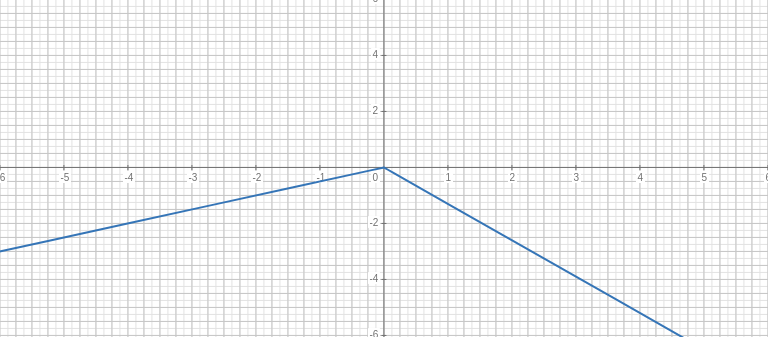
\includegraphics[width=1\textwidth ,scale=1]{funcion_matemapli.png}
\end{figure}

Sea $x_0 = 0.6$, como $x_0 > 0$ se tiene que $x_1 = f(x_0) = -\alpha x$. Definimos la solución general de la ecución en diferencias $x_{n+1} = -\alpha x_n$, cuyo polinomio característico es $P(\lambda)=\lambda + \alpha$ donde $P(\lambda) = 0 \Leftrightarrow \lambda = -\alpha$, luego la solución general sería $x_{n} = c_0\cdot(-1.3)^n$, teniendo en cuenta que el dato inicial es $x_0 = 0.6$ se tendría que $c_0 = 0.6$, luego $x_{n} = (0.6)\cdot(-1.3)^n$. Esta solución claramente alterna terminos, luego $x_1 < 0$. Por tanto $x_2 = f(x_1) = \beta x_1$, luego definiremos una segunda ecuación en diferencias cuyo valor inicial será $y_0 = -0.78 = 0.6\cdot(-1.3)$. $y_{n+1} = \beta y_n$ donde el polinomio característico asociado es $P(\lambda)= \lambda - \beta$ y se verifica que $P(\lambda) = 0 \Leftrightarrow \lambda = \beta$ y como el dato inicial es $y_0 = x_1 = -0.78$ se tiene que $y_{n} = -0.78\cdot(0.5)^n$ que es menor que cero $\forall n \in \mathbb{N}$, luego a partir de $x_1$ se sigue la ecuación en diferencias anterior donde es claro que,

\begin{equation*}
\lim_{n \to \infty} y_n = 0
\end{equation*}

luego como a partir de $x_1$ todos los términos son menores que 0 se verifica las segunda ecuación en diferencias y para el datos $x_0 = 0.6$ las soluciones tienden a 0 por la izquierda. \\ \\

Sea $x_0 = -0.8$, entonces como $x_0 < 0$ tendremos que $x_1 = f(x_0) = \beta x_0$. Definimos la solución de la ecuación en diferencias $x_{n+1} = \beta x_n$, cuyo polinimio característico asociado es $P(\lambda) = \lambda - \beta$ donde $P(\lambda)= 0 \Leftrightarrow \lambda = \beta$ luego como $x_0 = -0.8$ se tiene que la solución general de la ecucación en diferencias para la condición inicial $x_0=-0.8$ es $x_{n+1} = (-0.8)\cdot(0.5)^n$ donde esta solución es claramente menor que 0 $\forall n \in \mathbb{N}$. Luego se sigue esta solución $\forall n \in \mathbb{N}$, que claramente verifica que,

\begin{equation*}
\lim_{n \to \infty} x_n = 0
\end{equation*}

Luego hemos visto que se verifica que para ambas condiciones iniciales que las soluciones tienden a 0. \\ \\

\textbf{Apartado 2:} Claramente $p=0$ es un punto de equilibrio pues $\alpha \cdot p = 0$ para cualquier $\alpha$.
Usando el apartado anterior vemos que si la condición inicial $x_0$ es un número positivo, sea cual sea, se verificará que $x_1$ es menor que 0, pues por hipótesis $\alpha > 0$, luego $-\alpha < 0$, y por consiguiente $x_0 \cdot -\alpha < 0$. Luego a partir de $x_1$ se utiliza la solución de la ecuación en diferencias $y_{n+1}=x_n \cdot (\beta)^n$, que sabemos que converge a 0 si y sólo si $\beta < 1$, además por hipótesis tenemos que $\beta > 0$. Si la condición inicial fuese negativa se trabaja directamente con la solución general de $x_{n+1}=x_n \cdot \beta$, que converge a 0 si y sólo si $\beta < 1$. Luego si $\alpha \in \mathbb{R}+$ y $0 < \beta < 1$, para cualquier punto de un entorno de 0 se verificará que al aplicar $x_{n+1} = f(x_n)$ $\lim_{n \to \infty} x_n = 0$, luego si $\alpha \in \mathbb{R}^+$ y $0 < \beta < 1$ el punto p=0 será asintóticamente estable. \\ \\

\textbf{Ejercicio 2:} Dado $\alpha > 0$, se considera la ecuación en diferencias:
\begin{equation*}
x_{n+1} = 1 - \alpha|x_n|
\end{equation*}

\begin{enumerate}
\item Para $\alpha = 0.4$, estudia gráficamente el comportamiento de las soluciones en función de su dato inicial $x_0 \in \mathbb{R}$.
\item Para $\alpha > 0$ determina el número de puntos de equilibrio de la ecuación en diferencias.
\item Estudia la estabilidad de los puntos de equilibrio para $\alpha = 1.3$.
\item Si $\alpha = 2$, comprueba que $\{-0.2,0.6\}$ es un 2-ciclo y estudia su estabilidad.
\end{enumerate}

\textbf{Solución:} Primero para facilitar el trabajo posterior defino $f(x) = 1 - \alpha|x|$ y desdoblamos lo anterior en una función por partes de la siguiente manera,

\begin{equation*}
f(x)= \left\{ \begin{array}{lcc}
             1 -\alpha x &   si  & x \geq 0 \\
             \\ 1 + \alpha x &  si & x < 0
             \end{array}
   \right.
\end{equation*}
\textbf{Apartado 1:} Teniendo en cuenta que en la ecuación en diferencias dada hay un valor absoluto desdoblamos esta en dos,
\begin{figure}
\centering
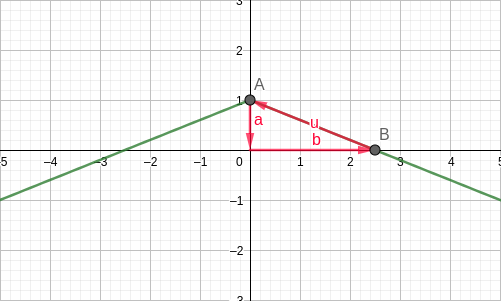
\includegraphics[width=0.8\textwidth, scale=1]{grafica_apar1.png}
\end{figure}
\begin{equation*}
x_{n+1}= \left\{ \begin{array}{lcc}
             1 -0.4 x_n &   si  & x \geq 0 \\
             \\ 1 + 0.4 x_n &  si & x < 0
             \end{array}
   \right.
\end{equation*}

, teniendo en cuanta lo anterior vamos a estudiar tres casos.

\begin{enumerate}
\item Si $0\leq x_n \leq 2.5$ tenemos que $0 \geq -0.4 x_n \geq -1$, de lo que obtenemos que $1 \geq 1-0.4 x_n \geq 0$. Como sabemos que $1-0.4x_n = x_{n+1}$, hemos demostrado que si $0 \leq x_n \leq 2.5 \Rightarrow 0 \leq x_{n+1} \leq 1$, pero como $x_{n+1}$ también verificará la hipótesis entonces $0 \leq x_{n+2} \leq 1$, y así sucesivamente para todo n+k con $k \in \mathbb{N}$. De aquí obtenemos que si $0 \leq x_0 \leq 2.5$ entonces $0 \leq x_n \leq 1$ para todo $n\in \mathbb{N}$. Para ver como se comportan las soluciones a largo plazo con esta condición inicial en primer lugar estudiamos si hay algún punto fijo. $\frac{1}{1.4}=\frac{5}{7} =x_*$ que es positivo y pertenece al intervalo [0,1]. Por consiguiente definimos la solución general de la ecuación en diferencias,

\begin{equation*}
P(\lambda) = \lambda+0.4 \Rightarrow P(\lambda) = 0 \Leftrightarrow \lambda = -0.4
\end{equation*}

De aquí hemos obtenido la solución de la ecuación homogénea asociada. Ahora como solución particular comamos $\frac{5}{7}$ llegando a $x_n = c_0\cdot(-0.4)^n + \frac{5}{7}$ cuyo limite verifica $\lim_{n \to \infty} x_n = \frac{5}{7}$. Y también se verifica que $c_0 = x_0 - \frac{5}{7}$. Y si $0 \leq x_0 \leq 2.5$ entonces $-\frac{5}{7} \leq c_0 \leq \frac{25}{14}$ y de aquí se obtiene que si $c_0$ verifica lo anterior entonces $x_n \geq 0$.

\item Segundo caso $x_n < 0$. Veamos que si $x_n < 0$ entonces $x_n < 0.4x_n < 0$ y claramente $x_n < 1+0.4x_n$. De aquí obtenemos que si $x_n < 0$, entonces existirá un $k \in \mathbb{N}$ tal que $x_n < x_{n+1} < ... < x_{n+k-1} < 0 < x_{n+k}$. Ahora tenemos que 
$x_{n+k-1}\cdot0.4 < 0 \Rightarrow 0 <1 + 0.4\cdot x_{n+k+1}=x_{n+k} < 1$. Como $0\leq x_{n+k} \leq 1$ aplicamos el caso anterior con $x_0 = x_{n+k}$. Luego si $x_0 < 0$ entonces existe un $k \in \mathbb{N}$ tal que $0 \leq x_k \leq 1$ y se aplica el caso anterior, es decir, $\lim_{n \to \infty} x_n = \frac{5}{7}$.

\item Tercer caso $x_n > 2.5$. De aquí se obtiene que $-0.4x_n < -1 \Rightarrow 1 -0.4x_n < 0$. Luego si $x_n > 2.5 \Rightarrow x_{n+1} < 0 \Rightarrow \exists k \in \mathbb{N} \> tal \> que \> 0\leq x_{n+1+k} \leq 1$. Luego si $x_0 > 2.5 \Rightarrow x_1 < 0$ entonces aplicamos el caso dos y finalmente el caso uno.
\end{enumerate}

De aquí hemos obtenido que independientemente de la condición inicial se tiende al punto de equilibrio que se encuentra en $\frac{5}{7}$. Fijándonos en la gráfica al principio del apartado si la condición inicial están en el cateto rojo b entonces $x_1$ permanecerá en el triángulo rojo. Si $x_0$ está por debajo del punto B, $x_1$ estará a la izquierda del eje y, y crecerá hasta entrar en el triángulo rojo. Si $x_0 < 0$, entonces $x_n$ crecerá hasta entrar en el triángulo rojo.

\textbf{Apartado 2:}Para realizar el estudio de los puntos de equilibrio estudiaremos dos casos:

\begin{itemize}
\item $x = 1 - \alpha x$, donde despejando la ecuación anterior se llega a $x = \frac{1}{1+\alpha}$. Como $\alpha > 0$ claramente $1 + \alpha > 0$ y por consiguiente $\frac{1}{1+\alpha}$, luego $p = \frac{1}{1 + \alpha}$ es un punto de equilibrio, para todo $\alpha > 0$.

\item $x = 1 + \alpha x$, donde despejando la ecuación anterior se llega a $x = \frac{1}{1 - \alpha}$. Para que el punto anterior sea de equilibrio se tiene que verificar que $\frac{1}{1 - \alpha} < 0$ luego se deberá verificar que $1 - \alpha < 0 \Rightarrow \alpha > 1$.
\end{itemize}

En conclusión, la función tendrá dos puntos de equilibrio si $\alpha > 1$, en caso contrario sólo tendra un punto de equilibrio. \\ \\

\textbf{Apartado 3:} Usando el apartado anterio como $\alpha > 1$ se tendran dos puntos de equilibrio, $p_1 = \frac{1}{1 + \alpha} = \frac{1}{2.3} \approx 0.43478$. Claramente la función f(x) es continua en el punto $p_1$ luego calcularemos la derivada.

\begin{equation*}
f'(x)= \left\{ \begin{array}{lcc}
             -1.3 &   si  & x \geq 0 \\
             \\ 1.3 &  si & x < 0
             \end{array}
   \right.
\end{equation*}

utilizando esta derivada vemos que $f'(p_1) \notin (-1,1)$, luego el punto de equilibrio $p_1$ no es asintóticamente estable. \\

Calculamos ahora $p_2 = \frac{1}{1-1.3}= \frac{1}{-0.3} \approx -3.33$ utilizando la derivada calculada para el caso anterior se tiene que $f'(p_2) \notin (-1,1)$, luego el punto de equilibrio $p_2$ tampoco es asintóticamente estable. Luego para $\alpha = 1.3$ ninguno de los puntos de equilibrio de la función es asintóticamente estable. \\ \\

\textbf{Apartado 4:} Probaremos que es un dos ciclo, luego $f(-0.2) = 1 + 2\cdot(-0.2) = 0.6$ y $f(0.6)= 1 - 2\cdot0.6 = -0.2$, luego queda demostrado que $\{-0.2,0.6\}$ es un 2-ciclo. Para ver que sea asintóticamente estable usaremos la regla de la cadena. Llamaremos $g(x) = 1 - \alpha x$ y $h(x) = 1 + \alpha x$. Luego,

\begin{equation*}
(g \circ h)'(-0.2) = g'(h(-0.2))\cdot h'(-0.2) = g'(0.6) \cdot 2 = -2 \cdot 2 = -4 \notin (-1,1)
\end{equation*}

si se compone $h \circ g$ al aplicar la regla de la cadena se ve a simple vista que $(h \circ g)'(0.6) = -4 \notin (-1,1)$ luego el 2-ciclo es claramente inestable. \\ \\

\end{document}
